%!TEX root = ../../main.tex
\section{Systemarkitektur}

I det følgende beskrives arkitekturen for systemet. Denne fungerer som vejledning og afgrænsning for udviklere på dette projekt. Hvis man vil viderudvikler på systemet er her et godt sted at starte med at få en basiside om projektets opbygning.\newline
Her beskrives systemets moduler i forskellige former for diagrammer. 

\begin{figure}[H]
	\centering
	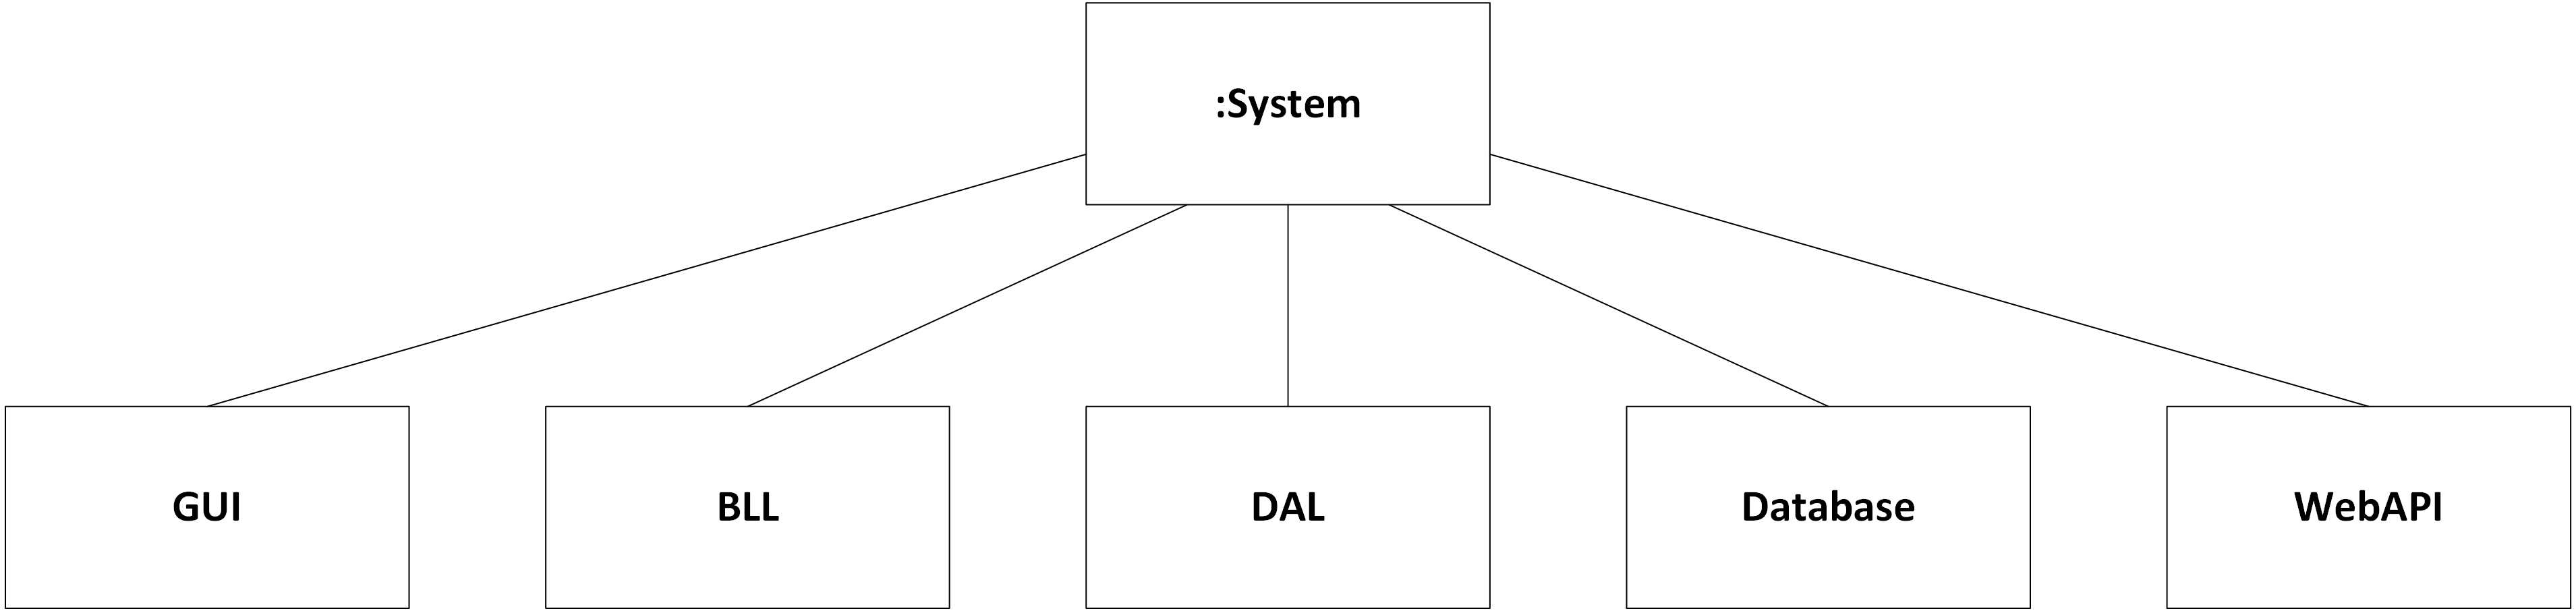
\includegraphics[scale=1.0]{Rapport/ArkitekturDiagram}
	\caption{Overordnet arkitekturdiagram}
	\label{ArkiDia}
\end{figure}

På figur \ref{ArkiDia} kan man se en overodnet opbygning af systemet. \textbf{GUI} er ansvarlig for interaktion med brugeren af systemet. Det er det som bartenderen ser ud ad til da han intet ved om systemets indre funktionalitet.\newline
\textbf{Business logikken} er al funktionaliteten i systemet. Her sker oprettelse af produkterm, salg og alt kommunikation med databasen. 
\textbf{Database} sørger for at gemme alt lige fra produkter og produktgrupper til salg og forskellige ordrer.\newline
\textbf{Web API} er frontend til at oprette, redigere og fjerne produkter. Her kan der også ses statistik over salg. Det er denne som admin bruger til at tilgå systemet. 

\subsection{N+1 view}

\subsubsection{Use Case View}
I dette view kan der ses hvordan de forskellige Use Cases bruger og omhandler systemet. Der er i dokumentationen indsat overordnede diagammer der beskriver handlindsforløbet for hver Use Case. Ydermere er der også lavet detaljerede sekvensdiagrammer der viser kommunikationen inde i systemet. \newline

\subsubsection{Logical View}
I Logical view kan der ses en oversigt over hvordan programmet er bygget op.
 


